\section{Exercises}
\subsection{Exercise 1}
\begin{quote}
\textit{
Familiarize yourself with the assembly language materials available on the 6.828 reference page. You don't have to read them now, but you'll almost certainly want to refer to some of this material when reading and writing x86 assembly.\\
We do recommend reading the section "The Syntax" in Brennan's Guide to Inline Assembly. It gives a good (and quite brief) description of the AT\&T assembly syntax we'll be using with the GNU assembler in JOS.
}
\end{quote}

该练习只是用于熟悉汇编语法,没有实际的内容

\subsection{Exercise 2}
\begin{quote}
\textit{
Use GDB's si (Step Instruction) command to trace into the ROM BIOS for a few more instructions, and try to guess what it might be doing. You might want to look at Phil Storrs I/O Ports Description, as well as other materials on the 6.828 reference materials page. No need to figure out all the details - just the general idea of what the BIOS is doing first.
}
\end{quote}

再次回忆一下BIOS的作用:BIOS作为保存在ROM中的特定位置的程序,在PC启动时被首先执行;在初始化一系列硬件环境之后,把bootloader从硬盘中导入内存并转移控制权。因此,Exercise 2中涉及到的代码即为“初始化硬件平台”相关的代码。

单就在QEMU中执行的代码而言,代码执行序列从指令\textsf{ljmp}开始,跳转到BIOS ROM中的低位指令并执行,一直到导入bootloader代码并跳转到其入口(0x7c00)为止。

Trace到的代码如下:\\

\begin{lstlisting}[language={[x86masm]Assembler}]
0xfe05b:	cmpl   $0x0,%cs:0x65b4
0xfe062:	jne    0xfd3aa
0xfe066:	xor    %ax,%ax
0xfe068:	mov    %ax,%ss
0xfe06a:	mov    $0x7000,%esp
0xfe070:	mov    $0xf431f,%edx
0xfe076:	jmp    0xfd233
0xfd233:	mov    %eax,%ecx
0xfd236:	cli    
0xfd237:	cld    
0xfd238:	mov    $0x8f,%eax
0xfd23e:	out    %al,$0x70
0xfd240:	in     $0x71,%al
0xfd242:	in     $0x92,%al
0xfd244:	or     $0x2,%al
0xfd246:	out    %al,$0x92
0xfd248:	lidtw  %cs:0x68f8
0xfd24e:	lgdtw  %cs:0x68b4
0xfd254:	mov    %cr0,%eax
0xfd257:	or     $0x1,%eax
0xfd25b:	mov    %eax,%cr0
0xfd25e:	ljmpl  $0x8,$0xfd266
\end{lstlisting}

首先,这段代码运行在16-bit实模式下。开始的几条指令只是简单的初始化一些寄存器的值,比如把栈指针\%esp的值赋成0x7000,以及禁用中断等操作。之后最关键的是:
\begin{enumerate}
\item I/O操作: 其中0x70与0x71是与CMOS交互,0x92是System Control Port;
\item 初始化GDT: 该指令是即将进入保护模式的前奏,因为保护模式的寻址方式与实模式完全不同,保护模式需要GDT;
\item 转换为保护模式: 直接把\%cr0设置为0x1即可
\end{enumerate}

有趣的一点是最后一条指令,为什么这里需要long jump?主要原因是,保护模式下无法按照原来的寻址模式找到应该要执行的段,必须查GDT表。

进入保护模式后的代码更加复杂,在这里不加赘述。

\subsection{Exercise 3}
\begin{quote}
\textit{Take a look at the lab tools guide, especially the section on GDB commands. Even if you're familiar with GDB, this includes some esoteric GDB commands that are useful for OS work.\\
Set a breakpoint at address 0x7c00, which is where the boot sector will be loaded. Continue execution until that breakpoint. Trace through the code in boot/boot.S, using the source code and the disassembly file obj/boot/boot.asm to keep track of where you are. Also use the x/icommand in GDB to disassemble sequences of instructions in the boot loader, and compare the original boot loader source code with both the disassembly in obj/boot/boot.asm and GDB.\\
Trace into bootmain()in boot/main.c, and then into readsect(). Identify the exact assembly instructions that correspond to each of the statements in readsect(). Trace through the rest of readsect()and back out into bootmain(), and identify the begin and end of the forloop that reads the remaining sectors of the kernel from the disk. Find out what code will run when the loop is finished, set a breakpoint there, and continue to that breakpoint. Then step through the remainder of the boot loader.}
\end{quote}

\subsubsection{Part 1}
执行调用bootmain()之前的代码。0x7c00是bootloader在内存中执行的起始地址,这时要执行的执行是在16-bit实模式下的cli指令:\\

\begin{lstlisting}
The target architecture is assumed to be i8086
[   0:7c00] => 0x7c00:	cli 
\end{lstlisting}
之后,在0x7c23的指令之前,所执行的操作包括:
\begin{enumerate}
\item 初始化段寄存器:CS,DS,SS
\item 启用A20线,这里采用的方法是用keyboard controller(加脚注)
\item 初始化全局描述符表(GDT),为转入保护模式做准备
\end{enumerate}

\begin{lstlisting}[language={[x86masm]Assembler}]
movl    %cr0, %eax
orl     $CR0_PE_ON, %eax
movl    %eax, %cr0
ljmp    $PROT_MODE_CSEG, $protcseg
\end{lstlisting}

当CR0被设置为0x1时,保护模式开启。注意这里的ljmp依然跟以前一样,为了跳转需要得到存储在全局描述符表中的段地址。

\subsubsection{Part 2}
对bootmain()的调用始于指令:\\

\begin{lstlisting}[language={[x86masm]Assembler}]
0x7c45:	call   0x7d0b 
\end{lstlisting}

经过调用gdb的x/i指令,以及分析boot.asm代码,发现0x7d0b是bootmain的起始地址,因此从值了开始调用bootmain()

bootmain()中主要进行的操作主要是把内核ELF文件load到指定的位置。为了完成这样一个功能,除了ELF格式提供的种种接口以外(包含在inc/elf.h)中,还需要readseg()函数来读取硬盘中的sector中的内容。readseg函数的定义:\\
\begin{lstlisting}
void readseg(uint32_t pa, uint32_t count, uint32_t offset) {
	uint32_t end_pa;
	end_pa = pa + count;
	pa &= ~(SECTSIZE - 1);
	offset = (offset / SECTSIZE) + 1;
	while (pa < end_pa) {
		readsect((uint8_t*) pa, offset);
		pa += SECTSIZE;
		offset++;
	}
}
\end{lstlisting}

该函数的了哟及并不复杂,给定要读取的数据大小count和起始位置offset以后,接下来需要的就是不断读取disk的一个sector的内容(因为sector是磁盘传输数据的最小单元),调用的函数是readsect(),定义如下:\\
\begin{lstlisting}
void readsect(void *dst, uint32_t offset) {
	waitdisk();

	outb(0x1F2, 1);		// count = 1
	outb(0x1F3, offset);
	outb(0x1F4, offset >> 8);
	outb(0x1F5, offset >> 16);
	outb(0x1F6, (offset >> 24) | 0xE0);
	outb(0x1F7, 0x20);	// cmd 0x20 - read sectors

	waitdisk();

	insl(0x1F0, dst, SECTSIZE/4);
}
\end{lstlisting}

该函数有很明显的“汇编特征”,下面是对其汇编代码的分析:

首先,waitdisk()函数被调用,目的是让程序等待磁盘可用,那如何得到该信息呢?通过观察waitdisk的asm代码,发现其首先调用inb从端口0x1f7读取一个byte的磁盘数据。该数据之后与0xC0求and,得到的是BSY和RDY位的信息,如果BSY位为真,则磁盘正处于忙状态。

当waitdisk()运行结束之后,此时disk可用,因此需要告诉磁盘要读的数据地址。关键是所有outb语句的最后一句outb(0x1F7, 0x20),其中0x1F7是磁盘I/O的端口,0x20是一条命令,用于读取sector(引用)

再次等待disk可用时,即可把disk对应位置的数据读入了,使用的指令是insl。这里要注意,被读入的地址在dst中。我在这里trace到了insl函数搜集到的数据,insl()内部包含一个循环,每次循环使用insl指令来读一个双字:

\begin{lstlisting}[language={[x86masm]Assembler}]
repnz insl (\%dx),\%es:(\%edi)
\end{lstlisting}
DX是端口号,ES是基址,EDI是偏移量寄存器。根据对循环的trace,发现ES在每次循环都不变,EDI增加4,即增加4个byte的偏移。即,读入了一个double word string。

bootloader首先读取的是ELF文件头,之后根据ELF文件的信息,把剩余的kernel代码导入。读入的目标内存地址存放在ELF的pa成员中。一旦ELF的所有数据都进入内存以后,执行kernel的入口函数:\\

\begin{lstlisting}
((void (*)(void)) (ELFHDR->e_entry))();
\end{lstlisting}
调用的是函数指针指向的函数。

\subsubsection{Part 3}

\begin{description}
\item[Question 1] \textit{At what point does the processor start executing 32-bit code? What exactly causes the switch from 16- to 32-bit mode?}

.code32之后的指令均为32位模式下的代码,但是之前当CR0被置0x1时已经进入32-bit的保护模式了

\item[Question 2] \textit{What is the last instruction of the boot loader executed, and what is the first instruction of the kernel it just loaded?} 

在调用内核入口函数的位置设置断点 b *0x7d63 后,得到bootloader的最后一条指令:\\

\begin{lstlisting}[language={[x86masm]Assembler}]
0x7d63:	call   *0x10018
\end{lstlisting}

很明显,0x10018是kernel入口函数的地址,之后跳转到这个函数。直接si就可以得到内核的第一条语句:\\
\begin{lstlisting}[language={[x86masm]Assembler}]
0x10000c:	movw   $0x1234,0x472
\end{lstlisting}

\item[Question 3] \textit{Where is the first instruction of the kernel?}

位置在0x10000c,不仅通过gdb可以trace到,在ELF Header中的start address也有提示。

\item[Question 4] \textit{How does the boot loader decide how many sectors it must read in order to fetch the entire kernel from disk? Where does it find this information?}

根据boot loader的程序逻辑:\\
\begin{lstlisting}
// load each program segment (ignores ph flags)
ph = (struct Proghdr *) 
    ((uint8_t *) ELFHDR + ELFHDR->e_phoff);
eph = ph + ELFHDR->e_phnum;
for (; ph < eph; ph++)
	readseg(ph->p_pa, ph->p_memsz, ph->p_offset);
\end{lstlisting}
由此可见,每次是对一个code segment调用readseg函数。ELF文件中清楚地指明了每个code segment的大小(p\_memsz)和起始位置(p\_offset)。

\end{description}


\subsection{Exercise 4}
\begin{quote} \textit{Exercise 4. Read about programming with pointers in C. The best reference for the C language is The C Programming Language by Brian Kernighan and Dennis Ritchie (known as 'K\&R'). We recommend that students purchase this book (here is an Amazon Link) or find one of MIT's 7 copies.\\
Read 5.1 (Pointers and Addresses) through 5.5 (Character Pointers and Functions) in K\&R. Then download the code for pointers.c, run it, and make sure you understand where all of the printed values come from. In particular, make sure you understand where the pointer addresses in lines 1 and 6 come from, how all the values in lines 2 through 4 get there, and why the values printed in line 5 are seemingly corrupted.\\
There are other references on pointers in C (e.g., A tutorial by Ted Jensen that cites K\&R heavily), though not as strongly recommended.\\
Warning: Unless you are already thoroughly versed in C, do not skip or even skim this reading exercise. If you do not really understand pointers in C, you will suffer untold pain and misery in subsequent labs, and then eventually come to understand them the hard way. Trust us; you don't want to find out what "the hard way" is.} \end{quote}

输出结果如下:\\
\begin{lstlisting}
1: a = 0x7fff576bf100, b = 0x7ffdd1c04bc0, c = 0x108540000
2: a[0] = 200, a[1] = 101, a[2] = 102, a[3] = 103
3: a[0] = 200, a[1] = 300, a[2] = 301, a[3] = 302
4: a[0] = 200, a[1] = 400, a[2] = 301, a[3] = 302
5: a[0] = 200, a[1] = 128144, a[2] = 256, a[3] = 302
6: a = 0x7fff576bf100,b = 0x7fff576bf104,c = 0x7fff576bf101
\end{lstlisting}

第1行和第6行是简单的C printf \%p标识符的用法:输出指针地址。2,3,4行很简单,主要考察的是指针指向同一个位置时,修改任意指针指向的值,都会影响其他指针指向的值(囧)。

第5行实际上是把c先类型转换为char型的指针,char型指针加1的结果,是指向的地址值加1(1byte)。之后再转换为int*类型后,c指向的位置是原始地址+1后的位置,对c的值的改变,会影响到a[1]的后3个byte和a[2]的第一个byte。

具体的计算:首先400的二进制形式为0b110010000,500的二进制形式为111110100,根据big-endian的规则,a[1]会变为0b11111010010010000,即低8位来自400,之后24位来自500的低24位。

\subsection{Exercise 5}
\begin{quote} \textit{Trace through the first few instructions of the boot loader again and identify the first instruction that would "break" or otherwise do the wrong thing if you were to get the boot loader's link address wrong. Then change the link address in boot/Makefragto something wrong, run make clean, recompile the lab with make, and trace into the boot loader again to see what happens. Don't forget to change the link address back and make cleanagain after} \end{quote}

如果链接地址不是在装载地址,那么很可能有些依赖于相对地址的跳转语句会跳转到奇怪的位置而出错。

把Makefrag中的-Ttext的值改为0x7C01,之后从0x7C00开始执行,可以发现:
\begin{enumerate}
\item 初始的几条指令均为nop;
\item continue之后在\lstinline{0x7c30:	ljmp   $0x8,$0x7c36}上出现错误了;
\end{enumerate}

\subsection{Exercise 6}
\begin{quote} \textit{We can examine memory using GDB's xcommand. The GDB manual has full details, but for now, it is enough to know that the command x/Nx ADDRprints Nwords of memory at ADDR. (Note that both 'x's in the command are lowercase.) Warning: The size of a word is not a universal standard. In GNU assembly, a word is two bytes (the 'w' in xorw, which stands for word, means 2 bytes).\\
Reset the machine (exit QEMU/GDB and start them again). Examine the 8 words of memory at 0x00100000 at the point the BIOS enters the boot loader, and then again at the point the boot loader enters the kernel. Why are they different? What is there at the second breakpoint? (You do not really need to use QEMU to answer this question. Just think.)} \end{quote}

在运行QEMU测试之前,首先想到运行到bootloader时和运行到kernel时的最大区别是:bootloader是加载到0x7C00的内存地址中,而kernel是加载到0x10000C的位置。因此前者不会影响0x100000之后的内存,而kernel会。

测试结果也是如此:
\begin{description}
\item[bootloader] address:\\
\lstinline{0x100000:	0x00000000	0x00000000	0x00000000	0x00000000}
\item[kernel] address:\\	
\lstinline{0x100000:	0x1badb002	0x00000000	0xe4524ffe	0x7205c766}\\
\lstinline{0x100010:	0x34000004	0x7000b812	0x220f0011	0xc0200fd8}\\
\lstinline{0x100020:	0x0100010d	0xc0220f80	0x10002fb8	0xbde0fff0}\\
\lstinline{0x100030:	0x00000000	0x117000bc	0x005fe8f0	0xfeeb0000}\\
\lstinline{0x100040:	0x53e58955	0x8b14ec83	0x5c89085d	0x04c70424}\\
\end{description}

\subsection{Exercise 7}
\begin{quote} \textit{Use QEMU and GDB to trace into the JOS kernel and stop at the movl \%eax, \%cr0. Examine memory at 0x00100000 and at 0xf0100000. Now, single step over that instruction using the stepiGDB command. Again, examine memory at 0x00100000 and at 0xf0100000. Make sure you understand what just happened.\\
What is the first instruction after the new mapping is established that would fail to work properly if the mapping weren't in place? Comment out the movl \%eax,\%cr0 in kern/entry.S, trace into it, and see if you were right.} \end{quote}

该指令的作用是启用32-bit保护模式,在此之前,\lstinline{0xf0100000}直接访问物理地址,而这已经超出了内存空间的范围,因此结果都是0;启用以后有了virtual memory机制,因此会把地址值\lstinline{0xf0100000}直接map到\lstinline{0x100000}的物理地址,所以读取改地址得到的内容和读取\lstinline{0x100000}的内容一样。

跟之前的Exercise 5很类似,这里注释掉以后,第一个利用了0xf01XXXXXX的地址的指令就会出错,这里是jmp(\lstinline{0x10002a})指令,因为其参数是\lstinline{0xf010002c}

\subsection{Exercise 7}
\begin{quote} \textit{We have omitted a small fragment of code - the code necessary to print octal numbers using patterns of the form "\%o". Find and fill in this code fragment} \end{quote}

直接按照10进制的写法修改即可。\\

即先用\lstinline{getuint}获取数值,然后设置base值为8,最后跳转到number标签进行处理:\\
\begin{lstlisting}
// (unsigned) octal
case 'o':
    num = getuint(&ap, lflag);
    base = 8;
    goto number;
\end{lstlisting}

输出:\lstinline{6828 decimal is 15254 octal!}

对后续问题的回答:

\begin{description}
\item[Question 1] \textit{Explain the interface between printf.c and console.c. Specifically, what function does console.c export? How is this function used by printf.c?}

printf.c使用了console.c提供的cputchar的实现。

根据注释,该函数的作用是提供一个high-level的对输出一个字符的功能的实现。

\item[Question 2] \textit{Explain the following from console.c}
\begin{lstlisting}
// What is the purpose of this?
if (crt_pos >= CRT_SIZE) {
    int i;

    memmove(crt_buf, crt_buf + CRT_COLS, 
        (CRT_SIZE - CRT_COLS) * sizeof(uint16_t));
    for (i = CRT_SIZE - CRT_COLS; i < CRT_SIZE; i++)
        crt_buf[i] = 0x0700 | ' ';
    crt_pos -= CRT_COLS;
}
\end{lstlisting}

该段代码是在一个往VGA buffer中填充一个字符的函数中。crt\_buf是缓冲区,CRT\_COLS是屏幕宽度,CRT\_SIZE是屏幕面积。因此,假如要输出的字符的位置已经超出当前屏幕大小限制时(即条件判断),要删掉上面一行并读取下面一行(即memmove),然后把屏幕上剩下的位置初始化(即最后的for循环)。

\item[Question 3] \textit{Trace the execution of the following code step-by-step}
\begin{lstlisting}
int x = 1, y = 3, z = 4;
cprintf("x \%d, y \%x, z \%d\n", x, y, z);
\end{lstlisting}
\begin{enumerate}
\item \textit{In the call to cprintf(), to what does fmt point? To what does ap point?}

fmt是格式化字符串,ap是参数列表。

\item[] \textit{List (in order of execution) each call to cons\_putc, va\_arg, and vcprintf. For cons\_putc, list its argument as well. For va\_arg, list what appoints to before and after the call. For vcprintf, list the values of its two arguments.}

cons\_putc的参数是参数列表的地址(即ap)\\
va\_arg用于根据类型移动位置\\
vcprintf的参数即为格式化字符串,以及参数列表(列表的地址可与cons\_putc的参数比较)\\

\end{enumerate}

\item[Question 3] \textit{Run the following code.\\
unsigned int i = 0x00646c72; cprintf("H\%x Wo\%s", 57616, \&i);}

结果是:He110 World

\item \textit{The output depends on that fact that the x86 is little-endian. If the x86 were instead big-endian what would you set ito in order to yield the same output? Would you need to change 57616 to a different value?}

57616的16进制表示即为e110,i的地址指针本来的类型为int *,这里因为\%s而转换为char *,造成的结果是分别对i的每个字节进行ASCII码的转换。和之前的问题一样,这里大端法小端法的结果一定不同。

\item[Question 5] \textit{n the following code, what is going to be printed after 'y='? (note: the answer is not a specific value.) Why does this happen?}

解释到y的时候已经超出参数列表的范围了,因此指向未分配的内存区域了。

\item[Question 6] \textit{Let's say that GCC changed its calling convention so that it pushed arguments on the stack in declaration order, so that the last argument is pushed last. How would you have to change cprintfor its interface so that it would still be possible to pass it a variable number of arguments?}

该问题肯定跟参数列表,或者说va\_arg的实现有关。通过grep找到在inc\/stdarg.h中有对应的实现:\\
\begin{lstlisting}
#define va_arg(ap, type) __builtin_va_arg(ap, type)
\end{lstlisting}
如果编译器改变了参数的顺序的话,在这里直接把函数的内容改成反方向的即可;比如原先是按照地址增长的顺序获得参数,现在可以按照减少的顺序获得

\end{description}

\subsection{Challenge} 
\begin{quote} \textit{Enhance the console to allow text to be printed in different colors. The traditional way to do this is to make it interpret ANSI escape sequences embedded in the text strings printed to the console, but you may use any mechanism you like. There is plenty of information on the 6.828 reference page and elsewhere on the web on programming the VGA display hardware. If you're feeling really adventurous, you could try switching the VGA hardware into a graphics mode and making the console draw text onto the graphical frame buffer.} \end{quote}

根据之前的题目分析可以发现,所有的VGA输出最后都要经过\lstinline{cga_putc}这个入口函数。该函数的参数是要输出的字符,加上格式化信息,即颜色。根据这一段代码:\\
\begin{lstlisting}
// if no attribute given, then use black on white
if (!(c & ~0xFF))
    c |= 0x0700;

switch (c & 0xff) {
    case '\b':
    if (crt_pos > 0) {
        crt_pos--;
        crt_buf[crt_pos] = (c & ~0xff) | ' ';
    }
    break;
    ...
\end{lstlisting}

很明显,因为后面的\lstinline{switch}取得仅有低8位,因此低8位是ASCII字符信息。那么颜色判断应该保存在前8位中。原代码中对颜色的处理很简单,只要当前位置没有字符,那么就输出黑色,否则不加颜色。

现在设置一个全局变量:\lstinline{user_vga_color},该值初始为0,用户可以用一些颜色宏来修改该值。定义如下颜色宏:\\
\begin{lstlisting}
#define VGA_COLOR_BLACK 1
#define VGA_COLOR_RED 4
#define VGA_COLOR_GREEN 2
\end{lstlisting}

并且修改\lstinline{cga_putc}函数:\\

同时在\lstinline{cga_init}中要初始化\lstinline{user_vga_color}为0\\
\begin{lstlisting}
c |= (user_vga_color << 8);

if (!(c & ~0xFF))
    c |= 0x0700;
\end{lstlisting}

想要输出颜色的时候可以直接:\\
\begin{lstlisting}
user_vga_color = VGA_COLOR_RED;
cprintf("RED");
\end{lstlisting}

输出结果如下图所示,在图片的最下方是输出的一条红字符串和一条绿字符串:\\
\begin{figure}[htbp] 
\centering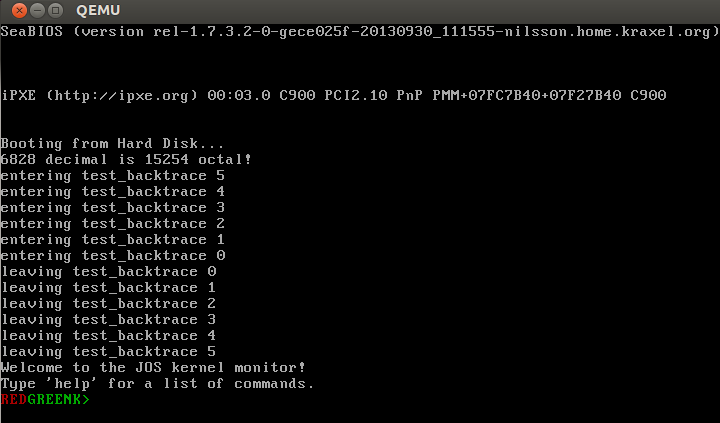
\includegraphics[width=5.5in]{Figure1} 
\caption{Challenge效果图}\label{fig:1} 
\end{figure} 


\subsection{Exercise 9.} 
\begin{quote} \textit{Determine where the kernel initializes its stack, and exactly where in memory its stack is located. How does the kernel reserve space for its stack? And at which "end" of this reserved area is the stack pointer initialized to point to?} \end{quote}

初始化栈一般是跟ESP(栈顶指针)寄存器有关。在entry.S中有如下语句:
\begin{lstlisting}[language={[x86masm]Assembler}]
# Set the stack pointer
movl	$(bootstacktop),\%esp
\end{lstlisting}

\lstinline{bootstacktop}是一个很神奇的值,观察下面一段在entry.S的结尾的代码:
\begin{lstlisting}[language={[x86masm]Assembler}]
.data
##################################################
# boot stack
##################################################
    .p2align	PGSHIFT		# force page alignment
    .globl		bootstack
bootstack:
    .space		KSTKSIZE
    .globl		bootstacktop   
bootstacktop:
\end{lstlisting}

这里声明了.data段,然后把栈底跟page的边界对齐(PGSHIFT是对齐变量),栈顶相对于栈底偏移了栈的大小(KSTKSIZE)。在inc/memlayout.h和inc/mem.h中定义了
\begin{enumerate}
\item PGSHIFT的大小为12,即$log_2(PGSIZE)$,PGSIZE为4096B,即4KB
\item KSTKSIZE的大小为page大小的8倍,即32KB
\end{enumerate}

因此\lstinline{bootstacktop}就是从data段开始的,对齐页边界以后,一个长度为32KB的栈的栈顶地址。把ESP初始化为该值以后,相当于得到了一个空栈。

下面检查一下\lstinline{bootstacktop}的值:首先objdump kernel发现.data的地址为\lstinline{0xf0110000},经过计算,\lstinline{bootstacktop}的值应该为\lstinline{0xf0118000}(该值在elf文件中也存在)。最后gdb调试时也发现\lstinline{bootstacktop}的值为\lstinline{0xf01180000}。


\subsection{Exercise 10.} 
\begin{quote} \textit{To become familiar with the C calling conventions on the x86, find the address of the test\_backtrace function in obj/kern/kernel.asm, set a breakpoint there, and examine what happens each time it gets called after the kernel starts. How many 32-bit words does each recursive nesting level of test\_backtrace push on the stack, and what are those words?\\
Note that, for this exercise to work properly, you should be using the patched version of QEMU available on the tools page or on Athena. Otherwise, you'll have to manually translate all breakpoint and memory addresses to linear addresses.} \end{quote}

\lstinline{test_backtrace}的起始地址在0xf0100040,之后执行的语句如下:\\

首先是对栈的操作和参数的处理:\\

\begin{lstlisting}[language={[x86masm]Assembler}]
f0100040:	55                   	push   %ebp
f0100041:	89 e5                	mov    %esp,%ebp
f0100043:	53                   	push   %ebx
f0100044:	83 ec 14             	sub    $0x14,%esp
f0100047:	8b 5d 08             	mov    0x8(%ebp),%ebx
\end{lstlisting}

ebp中存储的是基址,因此要将其入栈,然后把当前的栈顶位置esp保存到ebp中。由于寄存器ebx的值在call之后也要被保存,因此这里多了一次push。之后减少栈指针值,然后把参数x(即存放在0x8(ebp)处的数据)传给ebx。\\

下面计算栈空间:\\

首先,因为在函数刚被调用时,执行了两次\lstinline{push}操作,因此实际上使用了8byte的栈空间;之后,因为要保存传给\lstinline{test_backtrace}的参数和eip的值(即返回地址),又需要8个byte的空间;除此以外,\lstinline{test_backtrace}还调用了打印函数\lstinline{cprintf},该函数有两个参数,一个是格式化字符串,一个是参数列表。因为编译器之前已经确定,这里调用\lstinline{cprintf}的参数列表只有一个值x,因此要为调用\lstinline{cprintf}预留8byte的空间用于传递参数。因此,传递参数最多用8byte。但是因为esp在代码中直接减去了0x14,因此在这里的预留空间应该为20bytes。

综上,总共需要的空间为: \lstinline{8+20+4=32},即为32KB大小的空间。

举例,第一次调用\lstinline{cprintf}的参数准备:
\begin{lstlisting}[language={[x86masm]Assembler}]
=> 0xf010004a:	mov    %ebx,0x4(%esp)
14 cprintf("entering test_backtrace %d\n", x);
(gdb) 
=> 0xf010004e:	movl   $0xf01017a0,(%esp)
0xf010004e 14 cprintf("entering test_backtrace %d\n", x);
(gdb) x/s 0xf01017a0
0xf01017a0:	 "entering test_backtrace %d\n"
\end{lstlisting}

注意\lstinline{0xf01017a0}中存储的数据(即为\lstinline{x/s 0xf01017a0}的输出)。

\subsection{Exercise 11.}
\begin{quote} \textit{Implement the backtrace function as specified above.} \end{quote}

实现代码如下:\\
\begin{lstlisting}
int
mon_backtrace(int argc, char **argv, struct Trapframe *tf)
{
    int i;
    uint32_t ebp, eip, args[5];
    cprintf("Stack backtrace:\n");
    ebp = read_ebp();
    while (ebp != 0x0)
    {
        eip = *((uint32_t *)ebp+0x1);
        for (i = 0; i < 5; i++)
            args[i] = *((uint32_t*) ebp+2+i);
        cprintf("  ebp %08x  eip %08x", ebp, eip);
        cprintf("  args %08x %08x %08x %08x %08x\n", 
                args[0], 
                args[1], 
                args[2], 
                args[3], 
                args[4]);
        ebp = *((uint32_t *)ebp);
    }
    return 0;
}
\end{lstlisting}

基本思路是,ebp中保存的是函数刚被调用时,esp指向的位置,即栈顶;栈顶再往地址高位依次保存:上层过程调用的的ebp,返回的地址eip,以及最大5个的参数列表。

\subsection{Exercise 12.}
\begin{quote} \textit{Exercise 12. Modify your stack backtrace function to display, for each eip, the function name, source file name, and line number corresponding to that eip.} \end{quote}

首先应该解决\lstinline{__STAB_*}是什么的问题

在kernel.ld中,存在对.stab段的描述:
\begin{lstlisting}
/* Include debugging information in kernel memory */
.stab : {
    PROVIDE(__STAB_BEGIN__ = .);
    *(.stab);
    PROVIDE(__STAB_END__ = .);
    BYTE(0)     /* Force the linker to allocate space
                for this section */
}
\end{lstlisting}
这是一个linker script文件,目的是对程序的不同段进行位置分配。那么在这里分配一个.stab段的目的,正是为了在其中嵌入debug信息。用objdump的-G选项可以输出该ELF文件的stab信息。比如我想知道和代码文件console.c相关的stab信息,可以直接:\\
\begin{lstlisting}
>i386-jos-elf-objdump -G obj/kern/kernel | grep "console.c"                                                                         
137    SO     0      2      f010019c 2816   kern/console.c
167    SOL    0      0      f01001a8 2816   kern/console.c
173    SOL    0      0      f01001b3 2816   kern/console.c
177    SOL    0      0      f01001ba 2816   kern/console.c
200    SOL    0      0      f010021e 2816   kern/console.c
204    SOL    0      0      f0100226 2816   kern/console.c
211    SOL    0      0      f0100246 2816   kern/console.c
215    SOL    0      0      f010024e 2816   kern/console.c
219    SOL    0      0      f0100266 2816   kern/console.c
245    SOL    0      0      f01003a6 2816   kern/console.c
249    SOL    0      0      f01003c3 2816   kern/console.c
261    SOL    0      0      f01003d8 2816   kern/console.c
265    SOL    0      0      f01003e5 2816   kern/console.c
290    SOL    0      0      f01004b8 2816   kern/console.c
334    SOL    0      0      f010059a 2816   kern/console.c
338    SOL    0      0      f01005a0 2816   kern/console.c
343    SOL    0      0      f01005ae 2816   kern/console.c
350    SOL    0      0      f01005f0 2816   kern/console.c
354    SOL    0      0      f0100604 2816   kern/console.c
\end{lstlisting}

其中最终要的是最后一列,即stabstr,可以用来输出我们需要的调试信息;第二列指的是该stab的类型,如果是SO则代表文件名,SLINE代表代码行号,FUN代表的是函数名称。更进一步的分析可以发现,与一个函数相关的stab信息,都是连续的:\\

\begin{lstlisting}
435 FUN    0      0      f0100717 3928  mon_help:F(0,1)
436 PSYM   0      0      00000008 3853  argc:p(0,1)
437 PSYM   0      0      0000000c 3944  argv:p(0,19)
438 PSYM   0      0      00000010 3957  tf:p(0,20)
439 SLINE  0      34     00000000 0      
440 SLINE  0      38     00000006 0      
441 SLINE  0      40     0000003e 0      
442 FUN    0      0      f010075c 3968  mon_backtrace:F(0,1)
443 PSYM   0      0      00000008 3853  argc:p(0,1)
444 PSYM   0      0      0000000c 3944  argv:p(0,19)
445 PSYM   0      0      00000010 3957  tf:p(0,20)
446 SLINE  0      60     00000000 0      
447 SLINE  0      64     00000007 0      
448 SOL    0      0      f010076f 2831  ./inc/x86.h
\end{lstlisting}

在代码文件中,mon\_help与mon\_backtrace距离就很近(这里mon\_kerninfo为什么会被提前我也不知道),在stab段中也是紧挨着的。同时,第5列的值,对于FUN类型的stab来说,是汇编代码中的地址,而且这些地址是非降序的,所以我们可以通过eip在第5列上的二分查找来得到需要的信息(相关的功能已经在stab\_binsearch中实现了,因此这里只需要调用API即可)。

明白了原理以后,后续的修改就很容易了:

首先,在debuginfo\_eip中增加对行号的支持:\\
\begin{lstlisting}
stab_binsearch(stabs, &lline, &rline, N_SLINE, addr);
if (lline <= rline)
    info->eip_line = stabs[lline].n_desc;
else
    return -1;
\end{lstlisting}

然后,在\lstinline{mon_backtrace}中增加格式化输出的支持:\\
\begin{lstlisting}
if (debuginfo_eip(eip, &info) != -1)
{
    cprintf("        %s:", info.eip_file);
    cprintf("%d: ",        info.eip_line);
    cprintf("%.*s",        info.eip_fn_namelen, 
                           info.eip_fn_name);
    cprintf("+%u\n",       eip-(uint32_t)info.eip_fn_addr);
}
\end{lstlisting}

最后,增加\lstinline{backtrace}的命令:\\[1cm]
\begin{lstlisting}
static struct Command commands[] = {
{ "help", 
  "Display this list of commands", 
   mon_help },
{ "kerninfo", 
  "Display information about the kernel", 
  mon_kerninfo },
{ "backtrace", 
  "Display information about the current call stack", 
  mon_backtrace},
};
\end{lstlisting}